%
% Frontmatter - Introducci�n. Los miembros del tribunal que juzgan los PFC's tienen muchas m�s memorias que leer, por lo que
%	agradecer�n cualquier detalle que permita facilitarles la vida. En este sentido, realizar una peque�a introducci�n,
%	comentar la organizaci�n y estructura de la memoria y resumir brevemente cada cap�tulo puede ser una buena pr�ctica
%	que permita al lector centrarse f�cilmente en la parte que m�s le interesa.
%

\chapter[Introduction]{
	Introduction
}

Computer Graphics is a discipline that creates graphics using a computer. Advances in computer graphics have had an impact on several media types such as for example, the movies and video games industry, civil engineering, etc.

Images are normally captured by optical devices; such as cameras, LIDAR, mirrors, lenses, etc. Rendering is the process of generating an image from a model, the \emph{scene}, by means of a computer. A scene contains information like geometry, lighting, etc. about a virtual scene.

Typically, polygonal modeling has been the approach followed for modeling objects in the scene, approximating their surfaces using polygons. Point-based graphics focuses on points as the fundamental representation of the surfaces instead of polygons (see \figurename~\ref{poly_comp}).

\begin{figure}[h]
	\centering
	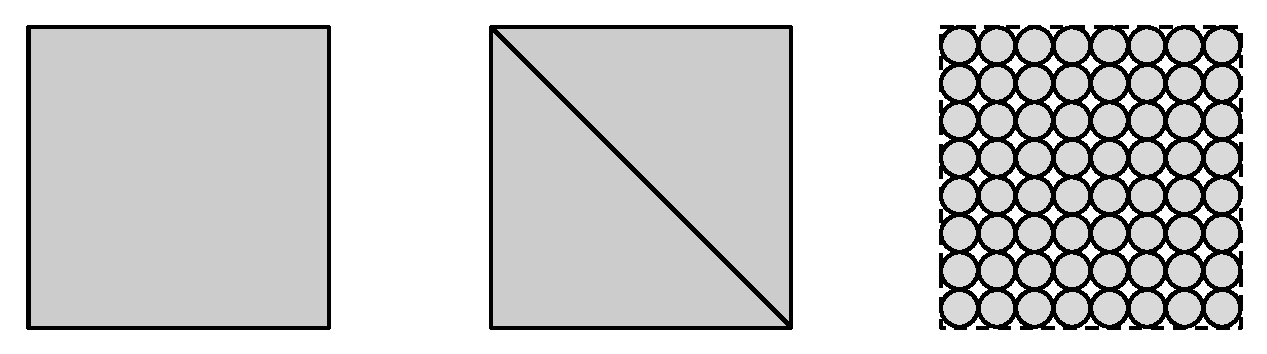
\includegraphics[scale=0.6]{eps/pol_comp.pdf}
	\caption[Modeling types comparison]{
		From left to right; mathematical representation of a plane, representation using two polygons (triangles) and a point-based representation.
	}
	\label{poly_comp}
\end{figure}

Using point based representations, the polygonal approximation step can be skipped and the massive amount of captured data is directly used.

All of these concepts will be explained in depth in their corresponding chapters. 

\section[Motivation and context]{
	Project motivation and context
}

Lately, 3D acquisition systems (commonly known as LIDAR\footnote{\textit{Laser Imaging Detection And Ranging}}) have evolved causing a revolution in work methodologies of several disciplines, from civil engineering, architecture, cultural heritage, movies to videogames. These systems use ultraviolet, visible or near infrared light to image objects. It can target a wide range of materials and even single molecules. A narrow laser beam can map features with very high precision.

Each sample obtained will possess coordinates (x,y,z), color, normal, temperature, etc. This information can be used to obtain measurements, calculations, etc. without having to repeat the capture process again each time we want to measure something new already present in the dataset. This presents clear advantages compared to the classical work-flow of a topographer that would have to measure on site each time a new measurement is required.       

PCM \cite{PCM} is a software library developed by the UDC\footnote{\textit{University of A Coru�a}} for the management of big point datasets obtained using LIDAR. PCM includes basic memory hierarchy management, making it possible to transfer the point cloud data between secondary memory (HDD) and video memory in the graphics card. PCM includes a very basic visualizer, that has the potential to become the seed for a more advanced point cloud software tool that will allow the user to access all of these features in real-time.   

Because of the massive nature of these datasets (some of them possess more than a billion points) achieving real-time manipulation of them is a complex task. It will require the improvement of PCM and a careful performance analysis. Having a system that is able to deal with these amounts of data, will let the user take advantage of the full precision of the capture devices if needed. 

Also because of the huge amounts of data, the possibility of using the massive parallel computing power of graphics cards will be explored. The large number of parallel processors can be used to reduce the computation times as much as possible. 

In this project, a complete software tool for visualization, management and manipulation of massive 3D point clouds will be developed. The tool will be multiplatform (GNU/Linux, Windows and MacOS) and will make use of open source software. That is why for the user interface it will take advantage of QT, that has native tools for all the aforementioned platforms. The resulting QT application will let the user access all of the functionality including an advanced and complete 3D visualizer.
   

\section[Objetives]{
	Project objetives
}

The aim of this project is the design and implementation of a point-based multiplatform software tool for interactive visualization, management and manipulation of massive 3D point clouds. 

The application will offer the user the necessary tools to work effectively with this type of datasets, including a 3D visualizer with advanced point-rendering techniques using OpenGL, that will allow real time interaction with one or multiple point clouds. 

From the interface, the user will be able to:     

\begin{itemize}
\item Select different visualization modes for point-based models: multiple cameras, simple and advanced visualization, multi-resolution, etc.
\item Combine different point clouds with tools that enable rotation, translation and scaling of the clouds.
\item Select points in the clouds for working with them.
\item Apply operations to a part of the cloud or the complete dataset. From simple operations like distance measurements to plane or other geometric primitives detection.
\item Export the work done to a standard CAD format, so the tool can be integrated in other workflows. 
\end{itemize}

The developed tool will take advantage of the parallel computing possibilities of the platforms. Either using the GPGPU capabilities of the graphics card with OpenCL or the multiple cores of the CPU. 

PCM will be used as the foundation for this work. PCM is a project in development that offers several low level tools for working with point clouds of arbitrary size in commodity hardware, from which a multi-resolution structure with different levels of cache is highlighted. This final year project will not only extend PCM with the mentioned features, offering a high level tool for the final user, but will also improve the existing source code; paying special attention to performance aspects.

\section[Structure]{
Document structure
}

 




